% 'draft' mode can be used to speed up compilation
\documentclass[twoside,final]{hcmut-report}
\usepackage{codespace}
\usepackage{fvextra}
\usepackage{graphicx}
\usepackage{titlesec}
\usepackage{algorithm}
\usepackage{algpseudocode}
\usepackage{tikz}
\usetikzlibrary{arrows.meta, matrix, positioning}
\setcounter{secnumdepth}{4}
% \usepackage[vietnamese,english]{babel}
\titleformat{\paragraph}
{\normalfont\normalsize\bfseries}{\theparagraph}{1em}{}
\titlespacing*{\paragraph}
{0pt}{3.25ex plus 1ex minus .2ex}{1.5ex plus .2ex}
\usepackage{subcaption}
\usepackage{float}
\usepackage{xurl}
% Draft watermark
% https://github.com/callegar/LaTeX-draftwatermark

% Encodings
\usepackage{gensymb,textcomp}

% Better tables
% Wide tables go to https://tex.stackexchange.com/q/332902
\usepackage{array,longtable,multicol,multirow,siunitx,tabularx}

% Better enum
\usepackage{enumitem}

% Graphics
\usepackage{caption,float}

% Add options for figures, like max width, framing, etc.
\usepackage[export]{adjustbox}

% References
% Use \Cref{} instead of \ref{}
\usepackage[nameinlink]{cleveref}

\usepackage{fontspec}
\usepackage{polyglossia}
\setmainlanguage{vietnamese}

% Chọn font có hỗ trợ tiếng Việt
\setmainfont{Times New Roman}

% FOR DEMONSTRATION PURPOSES, REMOVE IN PRODUCTION
\usepackage{mwe}


\DefineVerbatimEnvironment{verbatim}{Verbatim}{breaklines,commandchars=\\\{\},codes={\catcode`\$=3\catcode`\_=8},formatcom=\color{black},fontsize=\small}


% Sub-preambles
% https://github.com/MartinScharrer/standalone

% Configurations
\coursename{\huge{Thực tập 1}}
\title{Phát triển Plugin IntelliJ để tự động sinh kiểm thử tích hợp cho Microservices Spring Boot sử dụng phân tích tĩnh dựa trên PSI và RAG}
\advisor{& TS. Nguyễn Quốc Minh &}
\stuname{%
  & Ủ Minh Quân - 2470691 
}

% Allow page breaks inside align* environment
%\allowdisplaybreaks{}

% Makes a lot of things blue, avoid at all costs
%\everymath{\color{blue}}

% Set depth of numbering for counters
\AtBeginDocument{\counterwithin{lstlisting}{section}}

% Rename some sections
%\AtBeginDocument{\renewcommand*{\contentsname}{Contents}}
%\AtBeginDocument{\renewcommand*{\refname}{References}}
%\AtBeginDocument{\renewcommand*{\bibname}{References}}

% Custom commands
%\newcommand*\mean[1]{\bar{#1}}

\begin{document}
\coverpage%

\tableofcontents
\listoffigures
\listoftables
% \lstlistoflistings{}

\clearpage

\section{Giới thiệu tổng quan về IoT}

\subsection{Định nghĩa}
Internet of Things (IoT) là một mô hình trong đó các thiết bị vật lý được kết nối với Internet và có khả năng thu thập, trao đổi cũng như xử lý dữ liệu. Những thiết bị này có thể là các cảm biến, thiết bị gia dụng, máy móc công nghiệp, phương tiện giao thông hoặc các hệ thống tự động khác. Thông qua việc tích hợp các công nghệ như cảm biến, mạng truyền thông, điện toán đám mây và trí tuệ nhân tạo, IoT cho phép các thiết bị hoạt động thông minh hơn và có khả năng tương tác với môi trường xung quanh.

Trong một hệ thống IoT, các thiết bị thường được trang bị cảm biến để thu thập dữ liệu từ môi trường như nhiệt độ, độ ẩm, ánh sáng, vị trí hoặc chuyển động. Dữ liệu này sau đó được truyền qua mạng đến các hệ thống xử lý trung tâm, nơi dữ liệu được lưu trữ, phân tích và sử dụng để đưa ra các quyết định hoặc hành động tự động. Ví dụ, trong một hệ thống nhà thông minh, cảm biến nhiệt độ có thể gửi dữ liệu đến hệ thống điều khiển để tự động điều chỉnh điều hòa nhằm duy trì nhiệt độ phù hợp.

Một đặc điểm quan trọng của IoT là khả năng kết nối giữa nhiều thiết bị khác nhau trong cùng một hệ thống. Các thiết bị này có thể giao tiếp trực tiếp với nhau hoặc thông qua các nền tảng trung gian như máy chủ hoặc dịch vụ đám mây. Điều này giúp tạo ra một hệ sinh thái thiết bị thông minh, trong đó các thành phần có thể phối hợp hoạt động để tối ưu hóa hiệu suất và nâng cao trải nghiệm của người dùng.

Ngoài ra, IoT còn đóng vai trò quan trọng trong việc chuyển đổi số của nhiều ngành công nghiệp. Nhờ khả năng thu thập dữ liệu theo thời gian thực và tự động hóa quy trình, IoT giúp doanh nghiệp tối ưu hóa hoạt động, giảm chi phí vận hành và nâng cao hiệu quả quản lý. Do đó, IoT không chỉ là một công nghệ kết nối thiết bị mà còn là nền tảng cho các hệ thống thông minh trong tương lai.
\subsection{Quy mô và tầm quan trọng}
Trong những năm gần đây, IoT đã phát triển với tốc độ rất nhanh và trở thành một trong những xu hướng công nghệ quan trọng nhất trên thế giới. Sự phát triển của Internet, mạng không dây, cảm biến giá rẻ và điện toán đám mây đã tạo điều kiện thuận lợi cho việc triển khai các hệ thống IoT trên quy mô lớn. Hiện nay, hàng tỷ thiết bị IoT đã được kết nối trên toàn cầu và con số này dự kiến sẽ tiếp tục tăng mạnh trong tương lai.

Quy mô của IoT không chỉ thể hiện ở số lượng thiết bị kết nối mà còn ở lượng dữ liệu khổng lồ được tạo ra mỗi ngày. Các thiết bị IoT liên tục thu thập dữ liệu từ môi trường và truyền dữ liệu đó đến các hệ thống xử lý. Những dữ liệu này có thể được phân tích để đưa ra các quyết định thông minh, dự đoán xu hướng hoặc tối ưu hóa hoạt động của hệ thống. Chính vì vậy, IoT đóng vai trò quan trọng trong việc thúc đẩy các công nghệ như phân tích dữ liệu lớn (Big Data), trí tuệ nhân tạo (AI) và học máy (Machine Learning).

Tầm quan trọng của IoT còn thể hiện ở khả năng cải thiện chất lượng cuộc sống và nâng cao hiệu quả trong nhiều lĩnh vực. Trong lĩnh vực y tế, IoT cho phép theo dõi sức khỏe bệnh nhân từ xa thông qua các thiết bị đeo thông minh. Trong lĩnh vực giao thông, IoT giúp quản lý lưu lượng xe, giảm ùn tắc và nâng cao an toàn giao thông. Trong sản xuất công nghiệp, IoT giúp giám sát máy móc, phát hiện sớm các sự cố và tối ưu hóa quy trình sản xuất.

Bên cạnh đó, IoT cũng đóng vai trò quan trọng trong quá trình xây dựng các thành phố thông minh (Smart City). Các hệ thống cảm biến và thiết bị IoT có thể được sử dụng để quản lý năng lượng, giám sát môi trường, quản lý giao thông và cung cấp các dịch vụ công hiệu quả hơn cho người dân. Nhờ đó, IoT góp phần nâng cao hiệu quả quản lý đô thị và cải thiện chất lượng cuộc sống của cộng đồng.
\subsection{Các lĩnh vực ứng dụng chính}
IoT được ứng dụng rộng rãi trong nhiều lĩnh vực khác nhau của đời sống và kinh tế. Một trong những lĩnh vực phổ biến nhất là nhà thông minh (Smart Home). Trong hệ thống nhà thông minh, các thiết bị như đèn, điều hòa, camera an ninh và thiết bị gia dụng có thể được kết nối với nhau và điều khiển từ xa thông qua điện thoại thông minh hoặc các trợ lý ảo. Điều này giúp người dùng quản lý ngôi nhà của mình một cách tiện lợi và tiết kiệm năng lượng.

Trong lĩnh vực công nghiệp, IoT được ứng dụng trong mô hình sản xuất thông minh (Smart Manufacturing) hay còn gọi là Công nghiệp 4.0. Các cảm biến và thiết bị IoT được lắp đặt trên máy móc để thu thập dữ liệu về tình trạng hoạt động, hiệu suất và mức tiêu thụ năng lượng. Dữ liệu này được phân tích để tối ưu hóa quy trình sản xuất, giảm thiểu thời gian ngừng máy và nâng cao năng suất.

Lĩnh vực nông nghiệp cũng đang được hưởng lợi lớn từ IoT thông qua các hệ thống nông nghiệp thông minh (Smart Agriculture). Các cảm biến có thể đo độ ẩm đất, nhiệt độ, ánh sáng và các yếu tố môi trường khác để hỗ trợ nông dân trong việc tưới tiêu, bón phân và quản lý cây trồng. Nhờ đó, năng suất cây trồng được cải thiện và việc sử dụng tài nguyên được tối ưu hóa.

Ngoài ra, IoT còn được ứng dụng trong các lĩnh vực như y tế, giao thông, năng lượng và quản lý đô thị. Trong y tế, các thiết bị IoT giúp theo dõi sức khỏe bệnh nhân liên tục và hỗ trợ chẩn đoán bệnh từ xa. Trong giao thông, các hệ thống IoT có thể giám sát phương tiện và tối ưu hóa hệ thống giao thông thông minh. Trong lĩnh vực năng lượng, IoT giúp quản lý lưới điện thông minh và tối ưu hóa việc sử dụng năng lượng.

Nhờ sự đa dạng trong ứng dụng, IoT đang trở thành một nền tảng công nghệ quan trọng cho sự phát triển của nhiều ngành công nghiệp và dịch vụ trong tương lai.
\subsection{Tại sao kiến trúc phần mềm quan trọng trong IoT}
Kiến trúc phần mềm đóng vai trò rất quan trọng trong việc xây dựng và vận hành các hệ thống IoT. Một hệ thống IoT thường bao gồm nhiều thành phần khác nhau như thiết bị cảm biến, mạng truyền thông, nền tảng xử lý dữ liệu và các ứng dụng người dùng. Nếu không có một kiến trúc phần mềm được thiết kế hợp lý, việc tích hợp và quản lý các thành phần này sẽ trở nên rất phức tạp.

Một trong những thách thức lớn của IoT là số lượng thiết bị rất lớn và liên tục tăng theo thời gian. Kiến trúc phần mềm cần được thiết kế để đảm bảo khả năng mở rộng (scalability), cho phép hệ thống có thể xử lý và quản lý hàng triệu thiết bị cùng lúc mà vẫn đảm bảo hiệu suất ổn định. Điều này đòi hỏi các giải pháp như điện toán đám mây, xử lý dữ liệu phân tán và các kiến trúc dịch vụ linh hoạt.

Ngoài ra, vấn đề bảo mật cũng là một yếu tố quan trọng trong các hệ thống IoT. Các thiết bị IoT thường thu thập và truyền tải những dữ liệu nhạy cảm, do đó hệ thống cần có các cơ chế bảo mật mạnh mẽ để bảo vệ dữ liệu khỏi các cuộc tấn công mạng. Kiến trúc phần mềm cần tích hợp các cơ chế xác thực, mã hóa và kiểm soát truy cập để đảm bảo an toàn cho hệ thống.

Một yếu tố khác cần được xem xét là khả năng tương thích giữa các thiết bị và nền tảng khác nhau. Trong thực tế, các thiết bị IoT thường đến từ nhiều nhà sản xuất và sử dụng các giao thức khác nhau. Kiến trúc phần mềm cần hỗ trợ khả năng tích hợp và giao tiếp giữa các thiết bị này để đảm bảo hệ thống hoạt động một cách hiệu quả.

Tóm lại, kiến trúc phần mềm là nền tảng quan trọng giúp hệ thống IoT hoạt động ổn định, an toàn và có khả năng mở rộng. Việc thiết kế một kiến trúc phần mềm phù hợp sẽ giúp các hệ thống IoT đáp ứng tốt các yêu cầu về hiệu suất, bảo mật và khả năng tích hợp, từ đó tạo ra những giải pháp công nghệ hiệu quả cho nhiều lĩnh vực khác nhau.

\section{Đặc tính kiến trúc trong IoT}

\subsection{Khái niệm đặc tính kiến trúc}

Trong kỹ nghệ phần mềm, quá trình thiết kế hệ thống đòi hỏi sự phân định rõ ràng giữa hai khía cạnh yêu cầu cốt lõi \cite{richards2020}:

\begin{itemize}
    \item \textbf{Functional Requirements:} Xác định các hành vi, quy trình nghiệp vụ và luồng dữ liệu mà hệ thống phải thực thi. Khía cạnh này giải quyết bài toán ứng dụng (ví dụ: thu thập và lưu trữ dữ liệu nhiệt độ theo chu kỳ).
    \item \textbf{Architectural Characteristics:} Còn được gọi là thuộc tính chất lượng hoặc yêu cầu phi chức năng, xác định các tiêu chuẩn vận hành mà hệ thống phải đạt được \cite{richards2020}. Khía cạnh này định hình cấu trúc nền tảng (ví dụ: khả năng duy trì độ trễ dưới 100ms khi xử lý 1 triệu kết nối đồng thời).
\end{itemize}

Việc phân lập này mang tính quyết định, bởi lẽ logic nghiệp vụ có thể được tái cấu trúc trong quá trình phát triển, nhưng kiến trúc nền tảng thì rất khó thay đổi sau khi hệ thống đã đi vào vận hành. Một quy trình thiết kế chuẩn mực phải tuân thủ trình tự: \textbf{Yêu cầu nghiệp vụ $\rightarrow$ Đặc tính kiến trúc $\rightarrow$ Mẫu kiến trúc $\rightarrow$ Công nghệ triển khai} \cite{richards2020}.

\subsection{Các đặc tính cốt lõi của hệ thống IoT}

Khác với phần mềm truyền thống, hệ thống IoT phải tương tác trực tiếp với phần cứng, do đó thiết kế kiến trúc phải đối phó với những giới hạn khắt khe hơn từ thế giới thực \cite{lea2018}. Dưới đây là 8 đặc tính cốt lõi mà bất cứ hệ thống IoT nào cũng cần phải có:

\subsubsection*{1. Scalability}
\begin{itemize}
    \item \textbf{Định nghĩa:} Năng lực của hệ thống trong việc duy trì hoặc gia tăng mức độ hiệu năng khi khối lượng công việc được mở rộng \cite{richards2020}.
    \item \textbf{Góc độ IoT đặc thù:} Quá trình mở rộng trong IoT diễn ra trên hai trục độc lập: số lượng kết nối duy trì trạng thái và thông lượng dữ liệu thu nhận.
    \item \textbf{Ví dụ thực tiễn:} Trong một hệ thống IIoT (Industrial IoT), kiến trúc có thể sử dụng Apache Kafka làm lớp đệm phân tán trước khi định tuyến dữ liệu đến các cụm xử lý luồng như Apache Spark \cite{databricks_johndeere}.
\end{itemize}

\subsubsection*{2. Reliability}
\begin{itemize}
    \item \textbf{Định nghĩa:} Khả năng hệ thống duy trì các chức năng được chỉ định trong những điều kiện nhất định và trong một khoảng thời gian xác định \cite{richards2020}.
    \item \textbf{Góc độ IoT đặc thù:} Đặc tính này bao hàm khả năng "tự chủ ngoại tuyến" tại các điểm biên. Thiết bị phải có khả năng tiếp tục vận hành các quy trình thiết yếu ngay cả khi mất kết nối mạng WAN với đám mây \cite{lea2018}.
    \item \textbf{Ví dụ thực tiễn:} Một Edge Gateway tại trạm biến áp tiếp tục đánh giá dữ liệu cảm biến dựa trên công cụ quy tắc cục bộ để kích hoạt rơ-le ngắt điện khẩn cấp khi phát hiện quá tải \cite{lea2018}.
\end{itemize}

\subsubsection*{3. Performance}
\begin{itemize}
    \item \textbf{Định nghĩa:} Mức độ đáp ứng của hệ thống về mặt thời gian và thông lượng khi thực thi các tác vụ \cite{richards2020}.
    \item \textbf{Góc độ IoT đặc thù:} Do tương tác trực tiếp với các quá trình vật lý, yêu cầu về hiệu năng thường đi kèm với các ràng buộc thời gian thực và thời hạn cứng.
    \item \textbf{Ví dụ thực tiễn:} Trong điều khiển robot phẫu thuật từ xa, độ trễ tín hiệu lệnh phải được đảm bảo nghiêm ngặt dưới ngưỡng 50ms để ngăn ngừa rủi ro vận hành vật lý \cite{lea2018}.
\end{itemize}

\subsubsection*{4. Security}
\begin{itemize}
    \item \textbf{Định nghĩa:} Năng lực bảo vệ dữ liệu và hệ thống khỏi sự truy cập, sửa đổi, hoặc phá hoại trái phép.
    \item \textbf{Góc độ IoT đặc thù:} Bề mặt tấn công mở rộng ra môi trường vật lý. Các thiết bị đầu cuối thường đặt tại các vị trí không được kiểm soát an ninh \cite{lea2018}.
    \item \textbf{Ví dụ thực tiễn:} Tích hợp các module phần cứng bảo mật (như TPM) để lưu trữ chứng chỉ khóa công khai (mTLS), đảm bảo không thể trích xuất khóa riêng tư để giả mạo danh tính trên mạng lưới \cite{lea2018}.
\end{itemize}

\subsubsection*{5. Maintainability}
\begin{itemize}
    \item \textbf{Định nghĩa:} Mức độ hiệu quả và dễ dàng khi tiến hành sửa đổi, nâng cấp phần mềm hoặc khắc phục sự cố \cite{richards2020}.
    \item \textbf{Góc độ IoT đặc thù:} Chu kỳ sống của phần cứng kéo dài từ 10 đến 15 năm tại các môi trường khó tiếp cận, đòi hỏi cơ chế cập nhật OTA (Over-The-Air) phải có độ tin cậy tuyệt đối \cite{lea2018}.
    \item \textbf{Ví dụ thực tiễn:} Triển khai kiến trúc bộ nhớ phân vùng kép trên vi điều khiển, cho phép thiết bị tự động khởi động lại bằng phân vùng chứa firmware cũ nếu bản cập nhật phát sinh lỗi \cite{lea2018}.
\end{itemize}

\subsubsection*{6. Interoperability}
\begin{itemize}
    \item \textbf{Định nghĩa:} Năng lực trao đổi và sử dụng thông tin giữa các hệ thống hoặc thành phần phần mềm có kiến trúc khác biệt.
    \item \textbf{Góc độ IoT đặc thù:} Sự phân mảnh nghiêm trọng về tiêu chuẩn công nghiệp đòi hỏi hệ thống phải đồng thời xử lý đa dạng các giao thức truyền thông như: MQTT, CoAP, Modbus, LoRaWAN \cite{lea2018}.
    \item \textbf{Ví dụ thực tiễn:} Sử dụng một Edge Gateway đóng vai trò bộ chuyển đổi giao thức, dịch các bản tin từ Modbus RTU và Profinet sang định dạng chuẩn hóa trước khi truyền qua MQTT tới máy chủ \cite{aws_siemens2019}.
\end{itemize}

\subsubsection*{7. Observability}
\begin{itemize}
    \item \textbf{Định nghĩa:} Mức độ mà trạng thái nội bộ của một hệ thống có thể được suy luận thông qua các dữ liệu đầu ra bên ngoài của nó \cite{garrison2017}.
    \item \textbf{Góc độ IoT đặc thù:} Khả năng truy cập trực tiếp (ví dụ: SSH) vào các thiết bị vi điều khiển bị hạn chế. Hệ thống telemetry phải được thiết kế sẵn để xuất log và metrics hữu ích.
    \item \textbf{Ví dụ thực tiễn:} Hệ thống cảnh báo không chỉ dựa trên trạng thái mất kết nối mà còn tương quan với dữ liệu viễn trắc trước đó (ví dụ: đường cong suy giảm điện áp pin) để phân loại nguyên nhân ngoại tuyến \cite{ms_rollsroyce}.
\end{itemize}

\subsubsection*{8. Energy Efficiency}
\begin{itemize}
    \item \textbf{Định nghĩa:} Tỷ lệ giữa hiệu suất hoạt động của hệ thống so với mức tiêu hao năng lượng.
    \item \textbf{Góc độ IoT đặc thù:} Các thiết bị đầu cuối vận hành bằng pin đòi hỏi kiến trúc truyền thông phải tối ưu hóa chu kỳ hoạt động (duty cycle) của bộ vi xử lý và module vô tuyến \cite{lea2018}.
    \item \textbf{Ví dụ thực tiễn:} Thay thế mô hình giao tiếp đồng bộ dựa trên HTTP bằng giao thức LPWAN (như LoRaWAN), cho phép thiết bị duy trì trạng thái ngủ sâu và chỉ thức giấc theo chu kỳ \cite{lea2018}.
\end{itemize}

\subsection{Sự đánh đổi giữa các đặc tính kiến trúc}

Việc tối ưu hóa đồng thời toàn bộ các đặc tính kiến trúc là bất khả thi về mặt toán học và vật lý. Kiến trúc sư phần mềm bắt buộc phải thực hiện các quyết định đánh đổi chiến lược dựa trên độ ưu tiên của nghiệp vụ \cite{richards2020}:

\begin{itemize}
    \item \textbf{Security vs. Performance:} Quá trình thiết lập phiên bảo mật (ví dụ: TLS handshake) và chi phí tính toán cho các thuật toán mã hóa có thể làm tăng độ trễ mạng. \textit{Phương pháp giảm thiểu:} Ứng dụng tăng tốc phần cứng \cite{lea2018}.
    
    \item \textbf{Reliability vs. Performance:} Trong giao thức MQTT, mức chất lượng dịch vụ cao nhất (QoS 2) đòi hỏi quy trình xác nhận 4 bước, dẫn đến giảm sút nghiêm trọng thông lượng mạng \cite{lea2018}. \textit{Phương pháp giảm thiểu:} Áp dụng định tuyến phân lớp (QoS 0/1 cho telemetry, QoS 2 cho lệnh điều khiển).
    
    \item \textbf{Scalability vs. Maintainability:} Việc phân rã hệ thống thành Microservices giải quyết tốt bài toán phân tải, nhưng làm tăng theo cấp số nhân độ phức tạp vận hành. \textit{Phương pháp giảm thiểu:} Tích hợp công cụ điều phối container (Kubernetes) và quy trình GitOps \cite{garrison2017}.
\end{itemize}

\subsection{Đặc tính kiến trúc dẫn dắt việc lựa chọn mẫu kiến trúc}

Quá trình định lượng và xếp hạng các đặc tính ưu tiên sẽ hình thành cơ sở logic để xác định mẫu kiến trúc chủ đạo \cite{richards2020}:

\begin{itemize}
    \item \textbf{Ưu tiên Performance (Độ trễ < 100ms) $\rightarrow$ Mẫu Edge-Cloud Hybrid:} Kiến trúc phân tán năng lực tính toán về phía Edge Computing là bắt buộc để triệt tiêu độ trễ đường truyền \cite{lea2018}.
    \item \textbf{Ưu tiên Scalability (> 100,000 thiết bị) $\rightarrow$ Microservices kết hợp EDA:} Kiến trúc Event-Driven Architecture đóng vai trò hấp thụ tải, trong khi Microservices mở rộng độc lập \cite{richards2020}.
    \item \textbf{Ưu tiên Energy Efficiency $\rightarrow$ EDA với giao thức bất đồng bộ:} Mô hình EDA loại bỏ hoàn toàn cơ chế lấy mẫu dữ liệu polling, tối đa hóa vòng đời nguồn cung cấp năng lượng \cite{lea2018}.
\end{itemize}

\vspace{1em}
\noindent\textbf{Ví dụ thực tiễn: Lựa chọn kiến trúc cho hệ thống bảo trì dự đoán điện gió ngoài khơi}

\textbf{1. Bối cảnh nghiệp vụ:} 
Một doanh nghiệp năng lượng cần triển khai hệ thống giám sát cho hàng trăm turbine ngoài khơi. Kênh giao tiếp duy nhất là mạng vệ tinh với băng thông hẹp, chi phí cao và độ trễ lớn \cite{ms_rollsroyce}.

\textbf{2. Đánh giá và ưu tiên Đặc tính kiến trúc:}
\begin{itemize}
    \item \textbf{Reliability:} Các quy trình an toàn phải vận hành tự chủ không phụ thuộc vào lệnh đám mây \cite{lea2018}.
    \item \textbf{Performance:} Việc phát hiện bất thường phải thực thi dưới 50ms, không thể chờ tín hiệu mạng vệ tinh \cite{lea2018}.
    \item \textbf{Scalability \& Bandwidth Efficiency:} Băng thông vệ tinh không cho phép truyền tải toàn bộ dữ liệu viễn trắc thô \cite{ms_rollsroyce}.
\end{itemize}

\textbf{3. Quyết định lựa chọn Mẫu kiến trúc:}
Mẫu \textbf{Edge-Cloud Hybrid} được chỉ định để giải quyết triệt để sự đánh đổi giữa 3 đặc tính trên \cite{lea2018}.

\textbf{4. Diễn giải giải pháp phân bổ:}
\begin{itemize}
    \item \textbf{Tại tầng Edge:} Thiết bị chạy Machine Learning cục bộ. Nếu phát hiện nguy hiểm, xuất lệnh ngắt với độ trễ < 10ms  \cite{lea2018}.
    \item \textbf{Tại tầng Cloud:} Tầng Edge chỉ gửi đi anomalies hoặc aggregated data, tiết kiệm 95\% băng thông. Cloud dùng để lưu trữ và huấn luyện lại Machine Learning  \cite{lea2018}.
\end{itemize}

\section{Software architecture patterns \& Trade-Off}
Trong hệ sinh thái IoT, không tồn tại một khuôn mẫu kiến trúc phần mềm vạn năng. Việc thiết kế tối ưu thực chất là một quá trình phân tích và ưu tiên các đặc tính hệ thống nhằm đưa ra những quyết định đánh đổi mang tính chiến lược và có mục đích.

\subsection{Layered Architecture}

\subsubsection{Mô tả hệ thống}
Layered Architecture tổ chức thực thể phần mềm thành các tầng logic nằm ngang tách biệt, tuân thủ nguyên tắc Separation of Concerns. Trong kiến trúc này, mỗi lớp đảm nhiệm một vai trò chuyên biệt và chỉ tương tác với lớp liền kề theo trục dọc (thường bao gồm các lớp như trong hình \ref{fig:layered_architecture}). Sự phân chia này tạo ra một ranh giới rõ ràng về trách nhiệm giữa các thành phần trong hệ thống.

\paragraph*{Sơ đồ kiến trúc}

\begin{figure}[H]
    \centering
    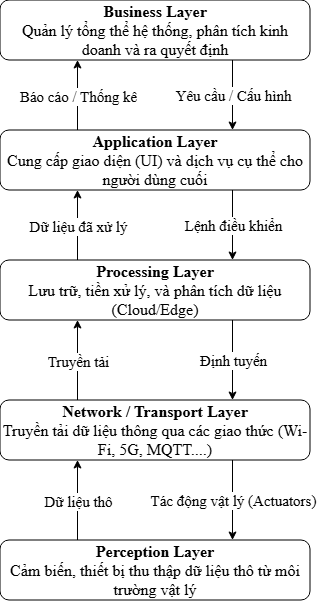
\includegraphics[width=0.4\linewidth]{graphics/LayeredArchitecture.drawio.png}
    \caption{Layered Architecture}
    \label{fig:layered_architecture}
\end{figure}

\subsubsection{Phân tích sự đánh đổi}
Ưu điểm lớn nhất là sự đơn giản trong tư duy thiết kế, giúp đội ngũ triển khai cực nhanh ở giai đoạn khởi tạo (Low entry barrier). Tuy nhiên, khi logic nghiệp vụ trở nên phức tạp, hệ thống có xu hướng biến tướng thành cấu trúc "Big Ball of Mud", gây khó khăn hệ trọng trong việc bảo trì và đọc hiểu mã nguồn. 

Mặc dù các thành phần trong cùng một lớp có tính đóng gói tốt, nhưng giữa các lớp lại tồn tại sự phụ thuộc chặt chẽ. Đặc biệt trong hệ sinh thái IoT, việc thay đổi một giao thức cảm biến mới thường gây ra "hiệu ứng vết dầu loang", buộc kỹ sư phải điều chỉnh mã nguồn đồng loạt trên nhiều tầng khác nhau.

Hạn chế về tính linh hoạt trong việc điều phối tài nguyên. Do các lớp liên kết theo chuỗi, khi tầng thu nhận dữ liệu bị quá tải, hệ thống buộc phải mở rộng toàn bộ ứng dụng thay vì chỉ tập trung vào thành phần đang bị bottleneck.

Kiến trúc này tối ưu cho các nhóm phát triển tinh gọn ($1-3$ người). Ngược lại, với các dự án quy mô lớn, việc phát triển song song thường dẫn đến xung đột luồng công việc và làm chậm tốc độ phân phối tính năng.

Bảng \ref{tab:layered-tradeoffs} dưới đây đúc kết các ưu điểm và hạn chế cốt lõi của mô hình Layered Architecture nhằm cung cấp cái nhìn tổng quan về khả năng vận hành của hệ thống.

\begin{table}[H]
\centering
\caption{Trade-off của Layered Architecture trong IoT}
\label{tab:layered-tradeoffs}
\begin{tabular}{|p{3.5cm}|p{5.5cm}|p{5.5cm}|}
\hline
\textbf{Tiêu chí} & \textbf{Ưu điểm} & \textbf{Nhược điểm} \\ \hline
\textbf{Tư duy thiết kế} & Đơn giản, Low entry barrier, giúp đội ngũ triển khai cực nhanh ở giai đoạn khởi tạo. & Dễ biến tướng thành "Big Ball of Mud" khi logic phức tạp, gây khó khăn lớn cho việc bảo trì và đọc hiểu. \\ \hline
\textbf{Coupling} & Các thành phần trong cùng một lớp có tính đóng gói rất tốt. & Phụ thuộc chặt chẽ giữa các lớp. Thay đổi ở một tầng (như giao thức cảm biến) dễ gây "hiệu ứng vết dầu loang". \\ \hline
\textbf{Điều phối tài nguyên} & Hỗ trợ tốt cho giai đoạn tập trung hiện thực hóa tính năng mà không bị quá tải bởi thiết lập hạ tầng. & Kém linh hoạt, phải mở rộng toàn bộ ứng dụng thay vì chỉ tập trung vào tầng đang bị quá tải (bottleneck). \\ \hline
\textbf{Hiệu năng \& Quy mô} & Tối ưu cho dự án PoC, Prototype, hệ thống nội bộ quy mô nhỏ (dưới 100 thiết bị). & Bị bottleneck khi vượt ngưỡng 1000 thiết bị. Không đáp ứng được Latency khắt khe dưới 100ms. \\ \hline
\textbf{Tổ chức đội ngũ} & Rất phù hợp và tối ưu cho các nhóm phát triển tinh gọn (1-3 người). & Dễ gây xung đột luồng công việc và làm chậm tốc độ phân phối tính năng khi phát triển song song ở dự án lớn. \\ \hline
\end{tabular}
\end{table}

\subsubsection{Ngữ cảnh áp dụng và Ngưỡng tới hạn}
Layered Architecture phát huy tối đa lợi thế trong các kịch bản ưu tiên tính tinh gọn như các dự án Proof of Concept (PoC), phiên bản thử nghiệm (Prototype), hoặc các hệ thống IoT nội bộ với quy mô quản lý dưới $100$ thiết bị. Ở giai đoạn này, cấu trúc phân lớp giúp đội ngũ tập trung vào việc hiện thực hóa tính năng mà không bị quá tải bởi các thiết lập hạ tầng phức tạp.

Tuy nhiên, kiến trúc này bắt đầu bộc lộ những hạn chế hệ trọng khi hệ thống tiến dần đến các ngưỡng vật lý và logic sau. Cụ thể, khi quy mô số lượng thiết bị vượt ngưỡng $1000$ node, khối lượng dữ liệu khổng lồ đi xuyên qua các lớp trung gian sẽ tạo ra bottleneck, khiến chi phí tài nguyên và công sức quản trị tăng theo hàm mũ. Bên cạnh đó, do đặc thù dữ liệu phải tuần tự đi qua từng tầng, kiến trúc này không thể đáp ứng các yêu cầu khắt khe về Latency dưới $100ms$ - một chỉ số sinh tử trong các ứng dụng IoT công nghiệp hoặc điều khiển tự động.

\subsubsection{Summary}
Layered Architecture đóng vai trò là giải pháp nền tảng giúp tối ưu hóa thời gian đưa sản phẩm ra thị trường trong các kịch bản có nguồn lực hạn chế và yêu cầu nghiệp vụ đơn giản. Tuy nhiên, do ràng buộc bởi Tight coupling và cơ chế xử lý tuần tự qua nhiều tầng, mô hình này bộc lộ các hạn chế về hiệu năng và quản trị khi hệ thống dịch chuyển sang quy mô lớn. Cụ thể, kiến trúc này gặp khó khăn trong việc mở rộng riêng lẻ các thành phần có tải cao. Ngoài ra, độ trễ tích lũy qua các lớp gây cản trở các tác vụ phản hồi nhanh trong IoT.

\subsection{Microservices Architecture}

\subsubsection{Mô tả hệ thống}
Microservices Architecture phân rã hệ thống IoT thành một tập hợp các đơn vị Independent Services với cơ chế Loose Coupling. Thay vì một khối mã nguồn duy nhất, hệ thống được module hóa dựa trên các phạm vi nghiệp vụ cụ thể như: Quản trị thiết bị, Thu nhận dữ liệu cảm biến, hoặc Xử lý sự kiện cảnh báo.

Đặc điểm cốt lõi của mô hình này nằm ở tính cô lập về dữ liệu và thực thi, mỗi dịch vụ toàn quyền quản lý cơ sở dữ liệu riêng biệt, giúp tránh tình trạng phụ thuộc chéo ở tầng lưu trữ. Việc trao đổi thông tin giữa các dịch vụ được thực hiện thông qua các API sử dụng giao thức mạng như REST, gRPC hoặc các hệ thống trung gian truyền tin (Message Broker) để đảm bảo tính phi tập trung của toàn hệ thống.

\paragraph*{Sơ đồ kiến trúc}

\begin{figure}[H]
    \centering
    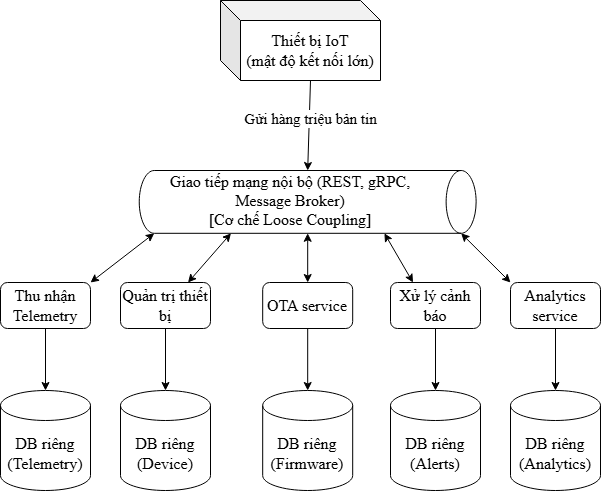
\includegraphics[width=0.9\linewidth]{graphics/MicroservicesArchitecture.drawio.png}
    \caption{Microservices Architecture}
    \label{fig:microservices_architecture}
\end{figure}

\subsubsection{Phân tích sự đánh đổi}
Việc chuyển đổi sang Microservices là một quyết định đánh đổi chiến lược, tập trung vào việc tối ưu hóa Elasticity và tính ổn định của hệ thống trên quy mô lớn. Ở khía cạnh lợi thế, kiến trúc này cung cấp Granular Scalability, cho phép điều phối tài nguyên độc lập dựa trên tải thực tế của từng dịch vụ. Điển hình là việc tăng cường năng lực xử lý cho tầng Telemetry Ingestion để tiếp nhận hàng triệu bản tin mà không gây lãng phí tài nguyên cho các dịch vụ có tần suất hoạt động thấp như OTA.

Song song đó, Fault Isolation giúp khu trú các sự cố tại một điểm (như dịch vụ Analytics) để ngăn chặn hiện tượng sụp đổ dây chuyền, mặc dù điều này đòi hỏi việc triển khai thêm các mẫu thiết kế phức tạp như Circuit Breaker hoặc Bulkhead để kiểm soát luồng thực thi.

Tuy nhiên, những ưu thế trên đi kèm với sự gia tăng đáng kể về Operational Complexity và các rào cản về hiệu năng. Hệ thống yêu cầu một hạ tầng quản trị tinh vi bao gồm Kubernetes, Service Mesh và Distributed Tracing, dẫn đến việc tiêu tốn một phần lớn nguồn lực kỹ thuật (ước tính từ $40\%$ đến $60\%$) cho công tác duy trì hạ tầng thay vì tập trung vào phát triển logic nghiệp vụ.

Bên cạnh gánh nặng về quản trị, Inter-service Latency phát sinh từ các bước Network hops giữa các dịch vụ cũng là một tham số kỹ thuật trọng yếu. Với độ trễ tích lũy dao động từ 10-30ms cho mỗi giao tiếp nội bộ, việc duy trì tổng thời gian phản hồi dưới 100ms trong các ứng dụng điều khiển IoT thời gian thực trở thành một thách thức lớn, đòi hỏi các giải pháp tối ưu hóa mạng hoặc chuyển đổi giao thức liên lạc một cách thận trọng.

Bảng \ref{tab:microservices-tradeoffs} dưới đây đúc kết các ưu điểm và hạn chế cốt lõi của mô hình Microservices Architecture nhằm cung cấp cái nhìn tổng quan về khả năng vận hành của hệ thống.

\begin{table}[H]
\centering
\caption{Trade-off của Microservices Architecture trong IoT}
\label{tab:microservices-tradeoffs}
\begin{tabular}{|p{3.5cm}|p{5.5cm}|p{5.5cm}|}
\hline
\textbf{Tiêu chí} & \textbf{Ưu điểm} & \textbf{Nhược điểm} \\ \hline
\textbf{Tính mở rộng} & Cung cấp Granular Scalability, cho phép mở rộng độc lập các dịch vụ có tải cao (như Telemetry Ingestion) mà không gây lãng phí tài nguyên. & Cần hạ tầng mạng và định tuyến phức tạp để hỗ trợ việc co giãn liên tục của các dịch vụ. \\ \hline
\textbf{Tính ổn định \& Cô lập lỗi} & Tính năng Fault Isolation giúp khu trú sự cố tại một điểm (vd: dịch vụ Analytics sập), ngăn chặn hiện tượng sụp đổ dây chuyền. & Phải triển khai thêm các mẫu thiết kế kiểm soát luồng phức tạp như Circuit Breaker hoặc Bulkhead. \\ \hline
\textbf{Độ phức tạp vận hành} & Tối ưu hóa Elasticity và tính ổn định của hệ thống trên quy mô lớn, hỗ trợ các đội ngũ độc lập làm việc song song. & Gia tăng đáng kể Operational Complexity. Tiêu tốn 40\%-60\% nguồn lực kỹ thuật chỉ để duy trì hạ tầng tinh vi (Kubernetes, Service Mesh, Tracing). \\ \hline
\textbf{Hiệu năng \& Latency} & Dịch vụ được phân rã giúp tối ưu hóa xử lý cho từng phạm vi nghiệp vụ cụ thể. & Phát sinh Inter-service Latency do Network hops (10-30ms/giao tiếp), gây thách thức lớn cho các ứng dụng IoT thời gian thực cần độ trễ dưới 100ms. \\ \hline
\end{tabular}
\end{table}

\subsubsection{Ngữ cảnh áp dụng và Ngưỡng tới hạn}
Hiệu quả thực thi của Microservices Architecture tỷ lệ thuận với quy mô thiết bị và năng lực quản trị vận hành của tổ chức. Kiến trúc này đạt đến trạng thái tối ưu trong các hệ sinh thái IoT công nghiệp có mật độ kết nối lớn (vượt ngưỡng $10.000$ thiết bị), nơi yêu cầu về sự phân rã dịch vụ trở nên cấp thiết để hỗ trợ các đội ngũ phát triển độc lập làm việc song song.

Ngược lại, mô hình này được xem là một lựa chọn không phù hợp đối với các doanh nghiệp khởi nghiệp ở giai đoạn sơ khởi, các nhóm kỹ thuật tinh gọn dưới $5$ nhân sự, hoặc những ứng dụng đặc thù yêu cầu độ trễ phản hồi cực thấp dưới ngưỡng $10ms$. Trong những kịch bản quy mô nhỏ hoặc yêu cầu thời gian thực khắt khe, gánh nặng về chi phí duy trì hạ tầng và độ trễ phát sinh từ giao tiếp mạng nội bộ sẽ triệt tiêu hoàn toàn các lợi ích về khả năng mở rộng, tạo ra một rào cản lớn đối với mục tiêu tối ưu hóa tài nguyên và tốc độ phân phối sản phẩm.

\subsubsection{Summary}
Tóm lại, Microservices Architecture là một giải pháp kiến trúc mang tính chiến lược nhằm giải quyết bài toán về quy mô và tính ổn định cho các hệ thống IoT phức tạp. Mặc dù cung cấp khả năng co giãn linh hoạt và cô lập lỗi hiệu quả, kiến trúc này đòi hỏi một sự đánh đổi nghiêm ngặt về hiệu năng mạng và nguồn lực vận hành hạ tầng. Việc quyết định áp dụng Microservices không chỉ đơn thuần là một lựa chọn kỹ thuật, mà còn là sự cân nhắc về mức độ trưởng thành của đội ngũ và yêu cầu đặc thù về độ trễ của hệ thống đích.

\subsection{Event-Driven Architecture - EDA}

\subsubsection{Mô tả hệ thống}
Event-Driven Architecture (EDA) là một mô hình kiến trúc phần mềm trong đó các thành phần của hệ thống giao tiếp với nhau thông qua các sự kiện (events). Trong kiến trúc này, các thành phần không tương tác trực tiếp với nhau thông qua các lời gọi hàm hoặc API đồng bộ, mà thay vào đó các thành phần sẽ phát sinh sự kiện khi có thay đổi trạng thái hoặc khi một hành động xảy ra. Các thành phần khác trong hệ thống có thể lắng nghe và phản ứng lại các sự kiện này.

Trong hệ thống IoT, Event-Driven Architecture đặc biệt phù hợp vì các thiết bị IoT thường liên tục tạo ra dữ liệu và các sự kiện từ môi trường. Ví dụ, một cảm biến nhiệt độ có thể tạo ra sự kiện khi nhiệt độ vượt quá một ngưỡng nhất định, hoặc một cảm biến chuyển động có thể phát sinh sự kiện khi phát hiện chuyển động trong khu vực được giám sát. Những sự kiện này sau đó được gửi đến hệ thống xử lý để kích hoạt các hành động tương ứng như gửi cảnh báo, lưu trữ dữ liệu hoặc điều khiển các thiết bị khác.

Một hệ thống EDA điển hình thường bao gồm một số thành phần chính. Thành phần đầu tiên là event producers, tức là các thành phần tạo ra sự kiện. Trong hệ thống IoT, các thiết bị cảm biến và thiết bị thông minh thường đóng vai trò là event producers vì chúng liên tục thu thập dữ liệu từ môi trường và phát sinh các sự kiện khi có thay đổi. Thành phần thứ hai là event broker hoặc event bus, có nhiệm vụ nhận và phân phối các sự kiện đến các thành phần khác trong hệ thống. Event broker đóng vai trò như một trung gian giúp các thành phần trong hệ thống có thể giao tiếp với nhau một cách linh hoạt mà không cần biết trực tiếp về nhau. Thành phần thứ ba là event consumers, tức là các thành phần nhận sự kiện và thực hiện các hành động tương ứng.

Trong nhiều hệ thống IoT hiện đại, các nền tảng xử lý sự kiện thường được triển khai trên các hệ thống phân tán hoặc các nền tảng điện toán đám mây. Các công nghệ như message queue hoặc hệ thống streaming dữ liệu thường được sử dụng để xử lý lượng lớn sự kiện được tạo ra từ các thiết bị IoT. Điều này cho phép hệ thống có thể xử lý dữ liệu theo thời gian thực và mở rộng khi số lượng thiết bị tăng lên.

Một đặc điểm quan trọng của Event-Driven Architecture là tính bất đồng bộ (asynchronous communication). Trong kiến trúc này, các thành phần không cần chờ phản hồi từ các thành phần khác sau khi gửi sự kiện. Điều này giúp giảm sự phụ thuộc giữa các thành phần và giúp hệ thống có thể xử lý nhiều sự kiện cùng lúc. Nhờ đó, EDA đặc biệt phù hợp với các hệ thống IoT có quy mô lớn và yêu cầu xử lý dữ liệu theo thời gian thực.

Ngoài ra, Event-Driven Architecture còn hỗ trợ việc xây dựng các hệ thống có khả năng mở rộng cao. Khi số lượng thiết bị IoT tăng lên, hệ thống có thể dễ dàng bổ sung thêm các thành phần xử lý sự kiện mà không cần thay đổi các thành phần hiện có. Điều này giúp hệ thống có thể thích nghi với sự phát triển nhanh chóng của các ứng dụng IoT.
Sơ đồ kiến trúc
\begin{figure}[H]
    \centering
    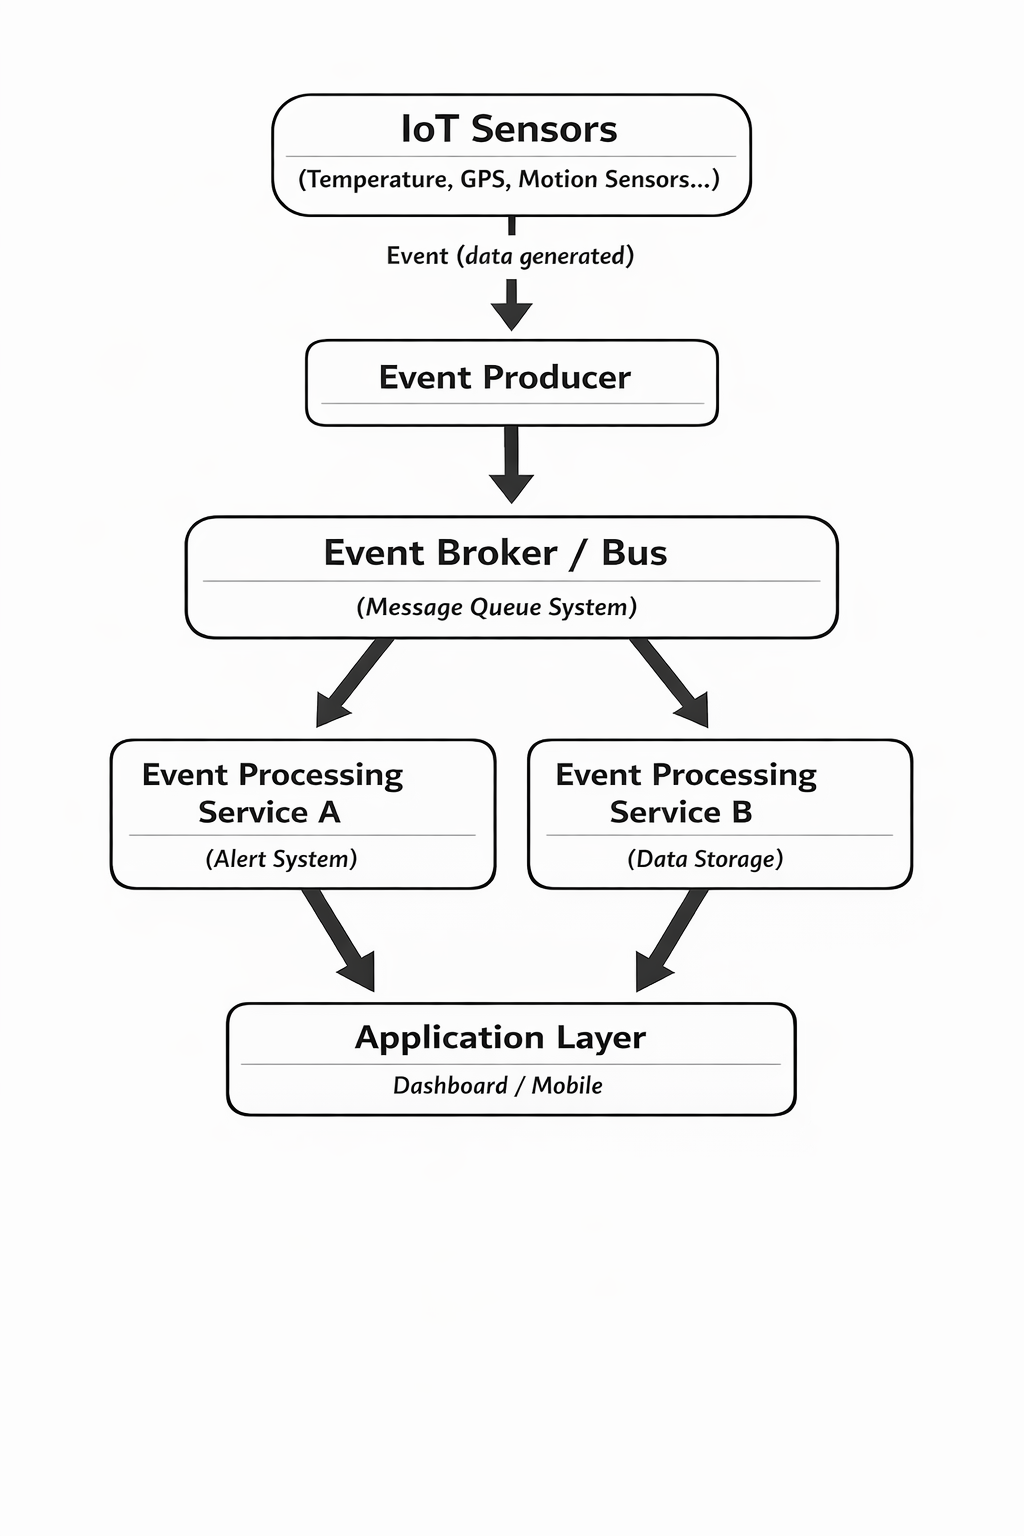
\includegraphics[width=0.5\linewidth]{graphics/EDA Architecture.png}
    \caption{Kiến trúc Event-Driven Architecture}
    \label{fig:placeholder}
\end{figure}

\subsubsection{Phân tích sự đánh đổi}

Mặc dù Event-Driven Architecture mang lại nhiều lợi ích cho các hệ thống IoT, việc áp dụng kiến trúc này cũng đi kèm với một số sự đánh đổi quan trọng. Việc hiểu rõ những trade-off này giúp các kiến trúc sư phần mềm có thể đưa ra quyết định phù hợp khi thiết kế hệ thống.

Một trong những lợi ích lớn nhất của Event-Driven Architecture là khả năng mở rộng (scalability). Do các thành phần trong hệ thống được tách rời và giao tiếp thông qua các sự kiện, hệ thống có thể dễ dàng mở rộng bằng cách thêm các thành phần xử lý sự kiện mới. Tuy nhiên, điều này cũng có thể làm tăng độ phức tạp của hệ thống, đặc biệt khi số lượng sự kiện và thành phần xử lý trở nên rất lớn. Việc theo dõi luồng dữ liệu và xác định nguyên nhân của các lỗi trong hệ thống có thể trở nên khó khăn hơn.

Một trade-off khác liên quan đến tính nhất quán dữ liệu (data consistency). Trong các hệ thống sử dụng Event-Driven Architecture, dữ liệu thường được xử lý theo mô hình bất đồng bộ. Điều này có thể dẫn đến tình trạng dữ liệu trong các thành phần khác nhau của hệ thống không được cập nhật ngay lập tức. Thay vì đạt được tính nhất quán tức thời, hệ thống thường áp dụng mô hình eventual consistency, trong đó dữ liệu sẽ trở nên nhất quán sau một khoảng thời gian nhất định.

Ngoài ra, Event-Driven Architecture cũng có thể tạo ra những thách thức trong việc quản lý và giám sát hệ thống. Khi các thành phần giao tiếp thông qua các sự kiện, việc theo dõi dòng chảy của dữ liệu và xác định vị trí xảy ra lỗi có thể trở nên khó khăn. Do đó, các hệ thống EDA thường cần các công cụ giám sát và logging mạnh mẽ để giúp phát hiện và xử lý sự cố.

Một yếu tố khác cần xem xét là độ trễ (latency) trong hệ thống. Trong một số trường hợp, việc xử lý sự kiện thông qua nhiều thành phần trung gian có thể làm tăng độ trễ của hệ thống. Điều này có thể ảnh hưởng đến các ứng dụng yêu cầu phản hồi nhanh. Vì vậy, khi thiết kế hệ thống EDA cho IoT, cần cân nhắc giữa lợi ích của kiến trúc bất đồng bộ và yêu cầu về hiệu suất của ứng dụng.

\begin{table}[h]
\centering
\caption{Trade-off của Event-Driven Architecture trong hệ thống IoT}
\begin{tabular}{|p{3.5cm}|p{6cm}|p{5.5cm}|}
\hline
\textbf{Tiêu chí} & \textbf{Ưu điểm} & \textbf{Nhược điểm} \\ \hline

Khả năng mở rộng (Scalability) 
& Hệ thống dễ mở rộng vì các dịch vụ hoạt động độc lập 
& Khi số lượng sự kiện quá lớn, cần hạ tầng mạnh để xử lý \\ \hline

Tính linh hoạt (Flexibility) 
& Có thể thêm hoặc thay đổi các dịch vụ xử lý sự kiện mà không ảnh hưởng hệ thống 
& Thiết kế hệ thống ban đầu phức tạp hơn \\ \hline

Khả năng phản ứng thời gian thực 
& Hệ thống có thể phản ứng nhanh với các sự kiện từ thiết bị IoT 
& Có thể phát sinh độ trễ nếu event pipeline quá dài \\ \hline

Tính tách rời (Decoupling) 
& Các thành phần không phụ thuộc trực tiếp vào nhau 
& Khó theo dõi luồng dữ liệu và debug hệ thống \\ \hline

Tính nhất quán dữ liệu 
& Hỗ trợ xử lý bất đồng bộ, phù hợp với hệ thống phân tán 
& Thường phải chấp nhận eventual consistency \\ \hline

Bảo trì hệ thống 
& Các dịch vụ có thể được phát triển và cập nhật độc lập 
& Cần hệ thống monitoring và logging phức tạp \\ \hline

\end{tabular}
\label{tab:eda_tradeoff}
\end{table}

\subsubsection{Ngữ cảnh áp dụng và Ngưỡng tới hạn}
Event-Driven Architecture đặc biệt phù hợp với các hệ thống IoT có đặc điểm tạo ra lượng lớn sự kiện từ các thiết bị cảm biến và yêu cầu xử lý dữ liệu theo thời gian thực. Trong những hệ thống như vậy, việc sử dụng mô hình giao tiếp đồng bộ có thể gây ra các vấn đề về hiệu suất và khả năng mở rộng. EDA giúp giải quyết vấn đề này bằng cách cho phép các thành phần giao tiếp thông qua các sự kiện và xử lý dữ liệu một cách bất đồng bộ.

Một trong những ngữ cảnh phổ biến nhất của EDA trong IoT là hệ thống giám sát và cảnh báo theo thời gian thực. Ví dụ, trong một hệ thống giám sát môi trường, các cảm biến có thể liên tục gửi dữ liệu về nhiệt độ, độ ẩm hoặc chất lượng không khí. Khi các giá trị này vượt quá ngưỡng cho phép, hệ thống có thể tạo ra sự kiện và kích hoạt các hành động như gửi cảnh báo đến người dùng hoặc kích hoạt các thiết bị điều khiển.

EDA cũng được sử dụng rộng rãi trong các hệ thống thành phố thông minh, nơi hàng nghìn hoặc hàng triệu thiết bị IoT được triển khai để thu thập dữ liệu về giao thông, năng lượng và môi trường. Trong những hệ thống này, các sự kiện được tạo ra liên tục và cần được xử lý nhanh chóng để hỗ trợ việc ra quyết định.

Ngoài ra, Event-Driven Architecture còn được áp dụng trong các hệ thống giám sát công nghiệp và bảo trì dự đoán (predictive maintenance). Các cảm biến được gắn trên máy móc có thể phát hiện các dấu hiệu bất thường và tạo ra sự kiện để cảnh báo cho hệ thống bảo trì trước khi xảy ra sự cố nghiêm trọng.

Tuy nhiên, Event-Driven Architecture không phải lúc nào cũng là lựa chọn tốt nhất cho mọi hệ thống. Trong các hệ thống nhỏ hoặc các ứng dụng có luồng xử lý đơn giản, việc sử dụng EDA có thể làm tăng độ phức tạp không cần thiết. Ngoài ra, đối với các hệ thống yêu cầu tính nhất quán dữ liệu ngay lập tức, kiến trúc event-driven có thể không phù hợp do bản chất bất đồng bộ của nó.

Một giới hạn khác của EDA là yêu cầu về hạ tầng công nghệ để xử lý và quản lý các sự kiện. Các hệ thống IoT quy mô lớn cần có các nền tảng xử lý dữ liệu và hệ thống message broker mạnh mẽ để đảm bảo hệ thống hoạt động ổn định. Việc triển khai và vận hành những hệ thống này có thể đòi hỏi chi phí và nguồn lực đáng kể.


\subsubsection{Summary}
Event-Driven Architecture là một mô hình kiến trúc phần mềm quan trọng và rất phù hợp với các hệ thống IoT hiện đại. Bằng cách sử dụng các sự kiện làm cơ chế giao tiếp giữa các thành phần, kiến trúc này cho phép hệ thống xử lý dữ liệu theo thời gian thực và mở rộng một cách linh hoạt khi số lượng thiết bị tăng lên.

Trong hệ thống IoT, Event-Driven Architecture thường bao gồm các thành phần như event producers, event broker và event consumers. Các thiết bị IoT đóng vai trò tạo ra sự kiện, trong khi các hệ thống xử lý dữ liệu và ứng dụng đóng vai trò tiếp nhận và xử lý các sự kiện này. Mô hình giao tiếp bất đồng bộ giúp giảm sự phụ thuộc giữa các thành phần và nâng cao khả năng mở rộng của hệ thống.

Tuy nhiên, việc áp dụng Event-Driven Architecture cũng đi kèm với một số trade-off như tăng độ phức tạp của hệ thống, khó khăn trong việc giám sát và quản lý dữ liệu, cũng như các vấn đề liên quan đến tính nhất quán dữ liệu. Do đó, việc thiết kế hệ thống EDA cần được thực hiện cẩn thận và kết hợp với các công cụ quản lý và giám sát phù hợp.

Trong bối cảnh các hệ thống IoT ngày càng phát triển và số lượng thiết bị kết nối ngày càng tăng, Event-Driven Architecture được xem là một giải pháp kiến trúc hiệu quả để xây dựng các hệ thống có khả năng mở rộng, linh hoạt và đáp ứng tốt các yêu cầu xử lý dữ liệu theo thời gian thực.

\subsection{Serverless Architecture}

Kiến trúc Serverless đang trở thành một trong những mô hình tiên quyết và phổ biến nhất để xử lý các workloads của hệ thống Internet of Things (IoT). Theo các nghiên cứu chuyên sâu về kiến trúc đám mây và báo cáo năng lực từ các nhà cung cấp (AWS, Azure), Serverless giải quyết hoàn hảo bài toán biến động dữ liệu (bursty traffic) vốn rất đặc trưng trong hệ thống thiết bị kết nối.

\subsubsection{Mô tả hệ thống}

Kiến trúc Serverless trong IoT hoạt động hoàn toàn dựa trên mô hình \textbf{Tính toán Hướng sự kiện (Event-Driven Compute)}. Trong mô hình này, không có máy chủ nào chạy nền chờ đợi lệnh. Toàn bộ mã nguồn nghiệp vụ chỉ được thực thi khi có một ``sự kiện'' cụ thể từ thiết bị phần cứng được đẩy lên đám mây.

\paragraph*{Sơ đồ kiến trúc}

\begin{figure}[H]
\centering
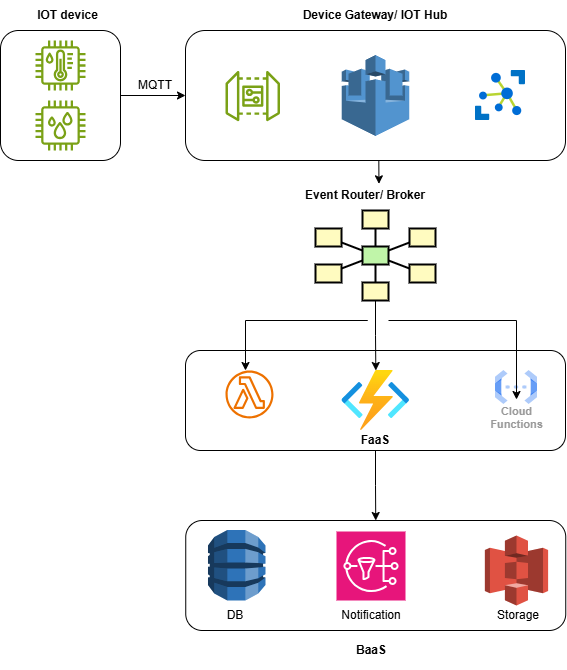
\includegraphics[width=0.9\textwidth]{graphics/serverless-architecture.png}
\caption{Sơ đồ kiến trúc Serverless IoT tiêu biểu}
\label{fig:serverless-architecture}
\end{figure}


\paragraph*{Các thành phần cốt lõi}

Cấu trúc cốt lõi của một hệ thống Serverless IoT bao gồm 4 thành phần chính:

\begin{enumerate}
    \item \textbf{Device Gateway / IoT Hub (Managed Service):}
    \begin{itemize}
        \item Đóng vai trò làm cổng giao tiếp, ví dụ như AWS IoT Core, Azure IoT Hub, Google Cloud IoT.
        \item Quản lý xác thực (Mutual TLS), duy trì kết nối hàng triệu thiết bị cùng lúc bằng các giao thức nhẹ như MQTT, CoAP.
    \end{itemize}

    \item \textbf{Event Router / Broker:}
    \begin{itemize}
        \item Khi thiết bị gửi một bản tin Telemetry hoặc cảnh báo, Broker sẽ đinhn tuyến bản tin này dựa trên các quy tắc sang các dịch vụ xử lý.
    \end{itemize}

    \item \textbf{FaaS (Function-as-a-Service):}
    \begin{itemize}
        \item Trái tim của hệ thống Serverless (ví dụ: AWS Lambda, Azure Functions, Google Cloud Functions).
        \item Mã nguồn được đóng gói thành các hàm nhỏ, phi trạng thái (stateless). Mỗi khi có sự kiện từ thiết bị, nền tảng Cloud sẽ tự động cấp phát một container chớp nhoáng, chạy hàm để xử lý dữ liệu, trả về kết quả và lập tức hủy container đó.
    \end{itemize}

    \item \textbf{BaaS (Backend-as-a-Service):}
    \begin{itemize}
        \item Các dịch vụ lưu trữ phụ trợ được quản lý 100\% như DynamoDB (NoSQL lưu trữ trạng thái thiết bị), Amazon S3 / Blob Storage (lưu trữ firmware), và các dịch vụ cảnh báo (SNS, Firebase Cloud Messaging).
    \end{itemize}
\end{enumerate}

\noindent\textbf{Luồng xử lý tiêu biểu:}\\
\texttt{Cảm biến Nhiệt độ} $\rightarrow$ \texttt{Gửi bản tin MQTT} $\rightarrow$ \texttt{IoT Hub Broker nhận bản tin} $\rightarrow$ \texttt{Kích hoạt hàm Lambda} $\rightarrow$ \texttt{Lambda xử lý, kiểm tra ngưỡng} $\rightarrow$ \texttt{Ghi log vào DynamoDB / Bắn cảnh báo SNS}.

% --------------------------------------------------
\subsubsection{Phân tích sự đánh đổi}
\label{subsec:serverless-tradeoff}

Serverless giải tỏa gánh nặng hạ tầng nhưng cũng buộc các Kiến trúc sư phải chấp nhận những hệ quả kỹ thuật nghiêm ngặt.

\begin{longtable}{c p{4cm} p{4cm} p{4cm}}

\caption{Phân tích đánh đổi kiến trúc Serverless trong IoT}\\

\toprule
\textbf{Chiều Đánh Đổi} & \textbf{Ưu điểm} & \textbf{Hạn chế} & \textbf{Bối cảnh IoT cụ thể} \\
\midrule
\endfirsthead

\toprule
\textbf{Chiều Đánh Đổi} & \textbf{Ưu điểm} & \textbf{Hạn chế} & \textbf{Bối cảnh IoT cụ thể} \\
\midrule
\endhead

\bottomrule
\endfoot

\textbf{Cost}
& \textbf{Pay-as-you-go \& Scale-to-Zero:} Chỉ trả tiền cho từng mili-giây xử lý dữ liệu. Rất hiệu quả cho các thiết bị gửi trạng thái thưa thớt.
& \textbf{Sustained Cost Penalty:} Ở tải liên tục cao, hóa đơn gọi hàm đắt gấp 3--10$\times$ so với Kubernetes/EC2 truyền thống.
& Công tơ nước đọc 1 lần/ngày: chi phí gần bằng 0. Telemetry liên tục 1M sự kiện/ngày: đắt hơn container 5--10$\times$. \\
\hline
\textbf{Latency}
& Phản hồi siêu nhanh đối với các hàm đã được khởi động sẵn (warm start $<$~10ms).
& \textbf{Cold Starts:} 100ms--2s để cấp phát môi trường khi hàm ngưng hoạt động lâu.
& Không chấp nhận được cho yêu cầu $<$~100ms (IIoT safety). Chấp nhận được cho cảnh báo có độ trễ 1--2s. \\
\hline
\textbf{Operations}
& \textbf{Zero Ops:} Không cần DevOps patch OS, tự động mở rộng hoàn hảo.
& \textbf{Vendor Lock-in:} Phụ thuộc sâu vào hệ sinh thái Cloud Provider. Không tinh chỉnh được phần cứng.
& Startup 2 người chạy alerting cho 10K thiết bị mà không cần DevOps. Di chuyển từ AWS sang Azure đòi viết lại IAM + function code. \\
\hline
\textbf{Scalability}
& Tự động scale từ 0 đến hàng triệu instance ngay lập tức.
& \textbf{Concurrency Limits:} AWS Lambda mặc định 1,000 concurrent executions/region. Có thể bị throttle khi spike đột ngột.
& Workload IoT bình thường. Toàn bộ fleet 50K thiết bị reconnect cùng lúc sau mất mạng $\rightarrow$ throttle hàng loạt. \\
\hline
\textbf{Quản lý Trạng thái}
& Bắt buộc thiết kế \textbf{Stateless}, giúp phục hồi sau gián đoạn tức thì. Tách biệt tính toán và dữ liệu.
& \textbf{Phức tạp luồng Stateful:} Theo dõi chuỗi sự kiện (VD: 3 lần vượt ngưỡng liên tiếp) cần Step Functions hoặc Redis bên ngoài.
& Theo dõi trạng thái thiết bị (alert đã gửi chưa?) cần DynamoDB/ElastiCache bên ngoài $\rightarrow$ thêm latency. \\
\hline
\textbf{Giới hạn thực thi}
& Thiết kế cho tác vụ ngắn $\rightarrow$ nhanh, gọn, dễ suy luận.
& AWS Lambda: tối đa 15 phút. Azure Functions: tối đa 10 phút. Không chạy được tác vụ dài.
& ML inference trên tập dữ liệu cảm biến lớn, video transcoding. Data enrichment nhẹ, routing, alerting. \\
\hline
\textbf{Quan sát \& Gỡ lỗi}
& Cloud tự động log cho mỗi lần thực thi (CloudWatch/Monitor).
& \textbf{Mê cung Debug:} Truy vết gói tin đi qua nhiều hàm phân tán rất khó. Cần Distributed Tracing (X-Ray).
& Chuỗi 5 hàm xử lý một alert $\rightarrow$ trace lỗi cần X-Ray/Jaeger. \\

\end{longtable}

% --------------------------------------------------
\subsubsection{Ngữ cảnh áp dụng và Ngưỡng tới hạn}
\label{subsec:serverless-thresholds}

Để kiến trúc tổng thể không rơi vào bẫy ``Anti-pattern'', cần rạch ròi giới hạn của Serverless.

\subsubsection*{Ngữ cảnh áp dụng lý tưởng}

\begin{enumerate}
    \item \textbf{Alerting Pipelines:}
    Mô hình lý tưởng nhất. Cảm biến báo cháy, cảm biến phát hiện rò rỉ hoặc phát hiện rung lắc. Hệ thống hầu như im lặng (Zero Cost) cho đến khi sự cố xảy ra, khi đó Serverless sẽ bung tối đa tài nguyên trong chốc lát để gửi hàng nghìn SMS/Email.

    \item \textbf{Tiền xử lý \& làm sạch dữ liệu:}
    Thiết bị gửi payload dạng chuỗi Hex hoặc Binary nén. Hàm Serverless nhận gói tin, giải mã, áp dụng chuẩn hóa (JSON Schema), và đẩy vào Data Lake hoặc Time-series DB.

    \item \textbf{Quản lý Vòng đời tự động:}
    Tự động chạy các kịch bản Provisioning, đăng ký chứng chỉ bảo mật (Certificates), hoặc cấu hình OTA Update khi thiết bị boot lần đầu tiên.
\end{enumerate}

\paragraph*{Ngưỡng tới hạn (Khi nào hệ thống Serverless sụp đổ?)}

\begin{table}[H]
\centering
\caption{Ngưỡng tới hạn của kiến trúc Serverless trong IoT}
\begin{tabularx}{\textwidth}{c X X X}
\toprule
\textbf{Ngưỡng} & \textbf{Giá trị tới hạn} & \textbf{Hậu quả khi vượt ngưỡng} & \textbf{Giải pháp thay thế} \\
\hline
\textbf{Latency}
  & Closed-loop control $<$~100ms
  & Cold Start (100ms--2s) vi phạm chuẩn an toàn vật lý (Safety-critical).
  & Chuyển sang \textbf{Edge Computing} hoặc container chạy thường trực. \\
\hline
\textbf{Throughput}
  & $>$~1M invocations/ngày liên tục 24/7
  & Chi phí Lambda vượt container 3--10$\times$. VD: Lambda $\sim$\$0.20/1M invocations + compute time vs Fargate $\sim$\$0.04/vCPU-giờ chạy liên tục.
  & Batching vào Kafka/Kinesis $\rightarrow$ xử lý bằng cụm Container (ECS/K8s). \\
\hline
\textbf{Thời gian thực thi}
  & $>$~15 phút (Lambda) / $>$~10 phút (Azure)
  & Timeout tự động ngắt tiến trình giữa chừng.
  & Tách thành pipeline Step Functions hoặc dùng Container/Batch. \\
\hline
\textbf{Concurrency}
  & $>$~1,000 concurrent executions (AWS mặc định)
  & Throttling hàng loạt khi toàn bộ fleet reconnect sau downtime hoặc DDoS.
  & Request quota increase trước hoặc dùng SQS queue làm buffer trước Lambda. \\
\hline
\end{tabularx}
\end{table}

% --------------------------------------------------
\subsubsection{Summary}
\label{subsec:serverless-summary}

Trong bức tranh kiến trúc IoT, \textbf{Serverless} là một ``vũ khí'' cực kỳ sắc bén, làm thay đổi hoàn toàn cục diện chi phí ban đầu và giải phóng đáng kể nguồn lực bảo trì hạ tầng của đội ngũ phát triển. Về cốt lõi, nó tận dụng sức mạnh đàn hồi của đám mây để xử lý các cơn sóng thần dữ liệu (data spikes) --- vốn là đặc tính cốt lõi của hoạt động phần cứng kết nối ngẫu nhiên.

Tuy nhiên, giới khoa học và các chuyên gia kiến trúc đều đồng thuận rằng: \textbf{Serverless KHÔNG phải là một ``Viên đạn bạc'' (Silver Bullet) có thể thay thế mọi thứ.}

\noindent\textbf{Dùng Serverless khi:}
\begin{itemize}
    \item Workload gián đoạn, bursty (cảnh báo, provisioning, ETL ngắt quãng)
    \item Đội ngũ nhỏ ($<$~3 người), không có DevOps
    \item Chi phí tối thiểu là ưu tiên hàng đầu
    \item Độ trễ 1--2s là chấp nhận được
\end{itemize}

\noindent\textbf{Không dùng Serverless khi:}
\begin{itemize}
    \item Telemetry liên tục tần suất cao ($>$~1M msg/ngày sustained)
    \item Safety-critical với yêu cầu $<$~100ms
    \item Tác vụ xử lý dài $>$~15 phút (ML training, video)
    \item Fleet lớn có nguy cơ reconnect storm
\end{itemize}

Sử dụng mô hình này như một mảnh ghép sắc bén ở lớp Xử lý Sự kiện bất đồng bộ, Cảnh báo và Tiền xử lý dữ liệu. Kế đến, họ sẽ điều tiết bằng cách giữ lại Container/Microservices dài hạn cho các luồng Ingestion lưu lượng lớn, và đặc biệt là áp dụng \textbf{Kiến trúc Edge Computing} cho bộ phận ra quyết định yêu cầu độ trễ $<$~100ms. Sự kết hợp khôn khéo này mới tạo nên một vóc dáng hệ thống IoT vững chãi và tối ưu thực sự.


\subsection{Edge-Cloud Hybrid Architecture}
\label{sec:edge-cloud-hybrid-deep-dive}

Kiến trúc Edge-Cloud Hybrid Architecture đang trở thành chuẩn mực thực tế (de-facto standard) cho các hệ thống IoT doanh nghiệp và Công nghiệp (IIoT). Bằng cách kết hợp sức mạnh phân tích vô hạn của Cloud Computing với khả năng phản hồi tức thì của Edge Computing, kiến trúc này giải quyết triệt để các hạn chế vật lý về độ trễ, băng thông mạng và tính liên tục trong vận hành.

% --------------------------------------------------
\subsubsection{Mô tả hệ thống}
\label{subsec:edge-cloud-system-description}

Kiến trúc Edge-Cloud Hybrid phân vùng trách nhiệm xử lý và lưu trữ dữ liệu thành 3 tầng phân cấp rõ rệt.

\paragraph*{Sơ đồ kiến trúc}

\begin{figure}[H]
\centering
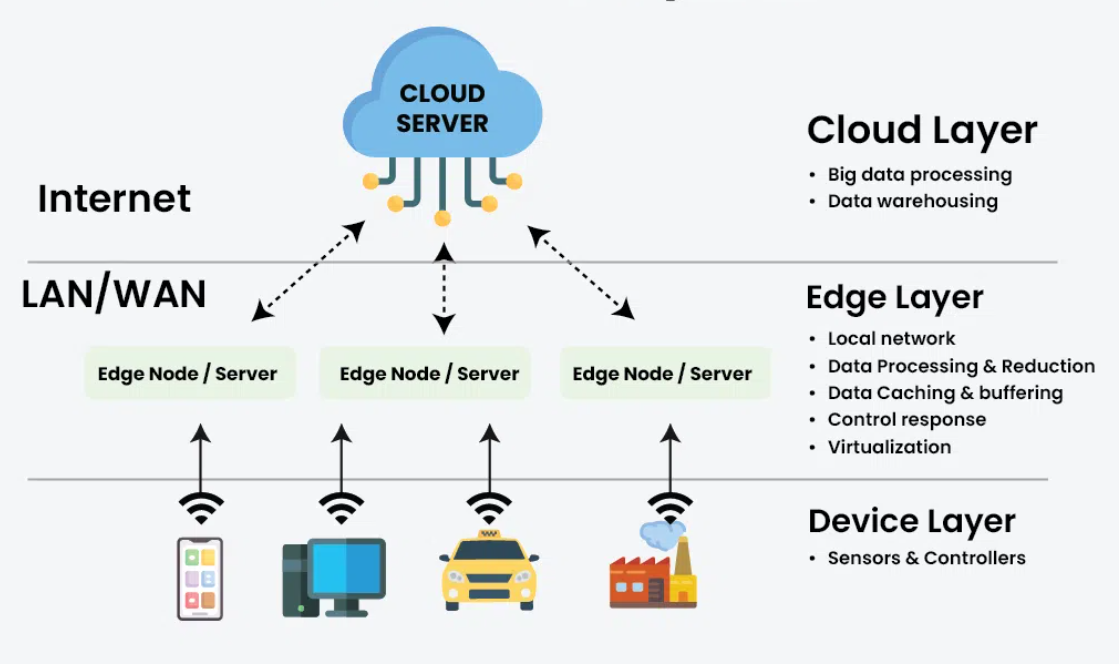
\includegraphics[width=0.9\textwidth]{graphics/Edge-Cloud-Architecture.png}
\caption{Sơ đồ kiến trúc Edge-Cloud Hybrid 3 tầng \cite{gfg_edge_cloud}}
\label{fig:edge-cloud-architecture}
\end{figure}

\paragraph*{Các thành phần cốt lõi}
\begin{enumerate}
    \item \textbf{Device Layer:}
    \begin{itemize}
        \item Các cảm biến, camera, PLC (Programmable Logic Controller) và cơ cấu chấp hành (actuators) ở điểm cực hạn. Chúng liên tục sinh ra lượng dữ liệu thô khổng lồ (Raw Data).
    \end{itemize}

    \item \textbf{Edge Layer:}
    \begin{itemize}
        \item Đóng vai trò là trung tâm thần kinh cục bộ. Phần cứng ở đây thường là các Industrial PC (IPC), Gateway, hoặc thiết bị nhúng mạnh mẽ (như NVIDIA Jetson).
        \item Chạy các phần mềm quản lý biên (như AWS IoT Greengrass, Azure IoT Edge).
        \item \textbf{Chức năng chính:} Tiền xử lý dữ liệu (lọc, nén, gộp), chạy quy tắc thời gian thực (Local Rules Engine), thực thi mô hình Machine Learning (AI Inference), và bảo mật cục bộ.
    \end{itemize}

    \item \textbf{Cloud Layer:}
    \begin{itemize}
        \item Đóng vai trò là trung tâm dữ liệu toàn cầu.
        \item \textbf{Chức năng chính:} Điều phối hàng triệu thiết bị, phân tích Big Data (Data Lake/Data Warehouse), huấn luyện mô hình ML (đưa các mô hình đã huấn luyện xuống Edge), và cung cấp Dashboard diện rộng.
    \end{itemize}
\end{enumerate}

\paragraph*{Cơ chế Đồng bộ hóa (Synchronization Patterns)}

\begin{table}[H]
\centering
\caption{Các cơ chế đồng bộ hóa trong kiến trúc Edge-Cloud Hybrid}
\begin{tabularx}{\textwidth}{c X X}
\toprule
\textbf{Cơ chế đồng bộ} & \textbf{Mô tả} & \textbf{Trường hợp sử dụng} \\
\hline
\textbf{Store-and-Forward}
  & Đệm dữ liệu cục bộ, gửi lên khi có kết nối.
  & Kết nối không ổn định (vệ tinh, 4G vùng sâu). \\
\hline
\textbf{Eventual Consistency}
  & Edge và Cloud hội tụ dần theo thời gian.
  & Telemetry không tới hạn (giám sát môi trường). \\
\hline
\textbf{Edge-First}
  & Edge tự ra quyết định, Cloud học từ kết quả.
  & Hệ thống an toàn thời gian thực (safety shutoff). \\
\hline
\textbf{Cloud-First}
  & Cloud ra quyết định, Edge thực thi lệnh.
  & Điều phối toàn bộ fleet (cập nhật firmware). \\
\hline
\textbf{Bi-directional Sync}
  & Cả Edge lẫn Cloud đều có thể thay đổi trạng thái.
  & Device Twin / Device Shadow (AWS/Azure). \\
\hline
\end{tabularx}
\end{table}

% --------------------------------------------------
\subsubsection{Phân tích sự đánh đổi}
\label{subsec:edge-cloud-tradeoff}

Triển khai Edge-Cloud là bài toán lớn về dòng tiền và năng lực kỹ thuật, đi kèm với những lợi thế và đánh đổi rõ rệt.

\begin{longtable}{c p{4cm} p{4cm} p{4cm}}

\caption{Phân tích đánh đổi kiến trúc Edge-Cloud Hybrid trong IoT} \\

\toprule
\textbf{Chiều Đánh Đổi} & \textbf{Ưu điểm} & \textbf{Hạn chế} & \textbf{Bối cảnh IoT cụ thể} \\
\midrule
\endfirsthead

\toprule
\textbf{Chiều Đánh Đổi} & \textbf{Ưu điểm} & \textbf{Hạn chế} & \textbf{Bối cảnh IoT cụ thể} \\
\midrule
\endhead

\bottomrule
\endlastfoot


\textbf{Latency}
  & Xử lý cục bộ: $<$~1ms on-device, $<$~10ms tại Edge Gateway.
  & Thêm một tầng kiến trúc cần quản lý và giám sát.
  & Ngắt khẩn cấp nhà máy không thể chờ round-trip Cloud (50--200ms); Edge phản ứng $<$~10ms. \\
\hline

\textbf{Reliability}
  & Tiếp tục vận hành khi Cloud không thể truy cập.
  & Đồng bộ sau khi kết nối lại rất phức tạp (conflict resolution, ordering, deduplication).
  & Nút lưới điện quản lý tải khi WAN bị ngắt. Dàn xếp 4 giờ sự kiện Edge với trạng thái Cloud cần thiết kế rất cẩn thận. \\
\hline

\textbf{Bandwidth}
  & Tổng hợp và lọc tại Edge --- chỉ gửi 1--5\% dữ liệu thô lên Cloud.
  & Phần cứng Edge (NVIDIA Jetson, IPC) tốn \$500--\$5,000+ mỗi site.
  & Nhà máy 500 camera: xử lý video tại Edge tiết kiệm 95\% băng thông Cloud. \\
\hline

\textbf{Data Sovereignty}
  & Dữ liệu nhạy cảm không bao giờ rời khỏi cơ sở.
  & Data residency đạt được bằng cấu hình, không phải kiến trúc --- cần kỷ luật vận hành.
  & Tuân thủ GDPR, HIPAA khi dữ liệu phải ở tại chỗ (on-premises / in-country). \\
\hline

\textbf{Security}
  & Phân đoạn mạng giới hạn bán kính tấn công khi bị xâm nhập.
  & Bảo mật vật lý Edge là trách nhiệm của nhà vận hành --- thiết bị có thể bị đánh cắp.
  & Kẻ tấn công có quyền truy cập vật lý vào Edge Gateway có thể trích xuất chứng chỉ Cloud backend. \\
\hline

\textbf{Complexity}
  & Công cụ phù hợp cho yêu cầu IoT doanh nghiệp phức tạp.
  & Mẫu phức tạp nhất --- cần chuyên môn về hệ thống phân tán, edge runtime (K3s, Greengrass), và giao thức đồng bộ.
  & Đội ngũ mới với IoT không nên bắt đầu từ đây --- đường cong học tập kéo chậm delivery hàng tháng. \\
\hline

\textbf{AI at the Edge}
  & ML inference trên thiết bị loại bỏ round-trip Cloud cho quyết định AI.
  & Cập nhật mô hình cần OTA delivery đến hàng nghìn node Edge.
  & YOLO object detection trên Jetson: 30fps cục bộ, không cần Cloud. Retrain và deploy mô hình mới đến 1,000 Edge node mất hàng giờ. \\

\end{longtable}

% --------------------------------------------------
\subsubsection{Ngữ cảnh áp dụng và Ngưỡng tới hạn}
\label{subsec:edge-cloud-thresholds}

Việc quyết định bao nhiêu phần trăm hệ thống đặt ở Edge và bao nhiêu phần đặt ở Cloud phụ thuộc vào các ngưỡng sau.

\paragraph*{Ngữ cảnh áp dụng lý tưởng}

\begin{enumerate}
    \item \textbf{Computer Vision \& Video Analytics:}
    Hàng trăm camera nhà máy đẩy video 4K sẽ đánh sập băng thông nội bộ. Edge Gateway chạy mô hình YOLO/SSD nhận diện lỗi ngay trên chuyền, chỉ gửi metadata (JSON): \texttt{\{"camera\_id": 04, "defect\_detected": "scratched\_surface", "timestamp": "..."\}}.

    \item \textbf{Cơ sở hạ tầng Thiết yếu \& Cận biên:}
    Gian khoan dầu ngoài khơi, tàu biển, mỏ khai thác sâu dưới lòng đất. Nơi kết nối vệ tinh đắt đỏ, chập chờn và dung lượng siêu thấp.

    \item \textbf{Tuân thủ Quyền riêng tư Y tế:}
    Hệ thống giám sát bệnh nhân trong phòng hồi sức. Dữ liệu nhịp tim phân tích tại giường bệnh, chỉ đẩy lên Cloud chỉ số sinh tồn đã ẩn danh hóa.
\end{enumerate}

\paragraph*{Ngưỡng tới hạn (Khi nào nên và không nên dùng Edge?)}

\begin{table}[H]
\centering
\caption{Ngưỡng tới hạn của kiến trúc Edge-Cloud Hybrid trong IoT}
\begin{tabularx}{\textwidth}{c X X X}
\toprule
\textbf{Ngưỡng} & \textbf{Giá trị tới hạn} & \textbf{Hậu quả khi vượt/không đạt ngưỡng} & \textbf{Giải pháp thay thế} \\
\hline
\textbf{Latency}
  & Ứng dụng yêu cầu $<$~50ms (closed-loop control).
  & Cloud-only bất khả thi --- round-trip Internet 50--200ms vi phạm chuẩn an toàn.
  & Edge \textbf{bắt buộc} cho vòng lặp kiểm soát. \\
\hline
\textbf{Bandwidth}
  & Ingestion rate $>$ năng lực uplink (VD: 10MB/s sinh ra vs 2MB/s uplink 4G).
  & Packet loss, queue overflow, hoặc hóa đơn Cloud bandwidth khổng lồ.
  & Triển khai Edge để nén, gộp (Batching) và chỉ gửi anomaly. \\
\hline
\textbf{Team Capability}
  & Đội ngũ chưa có kinh nghiệm hệ thống phân tán.
  & Lỗi đồng bộ (double-execution, lost updates) rất tinh vi và thảm khốc. Rollout OTA sai có thể brick hàng nghìn thiết bị.
  & Bắt đầu với Cloud-only + Rules Engine đơn giản. Thêm Edge khi đội ngũ trưởng thành. \\
\hline
\textbf{CapEx / ROI}
  & Dữ liệu giá trị thấp + Cloud bandwidth đủ rẻ.
  & Thêm Edge phức tạp hóa kiến trúc mà không mang lại lợi ích tương xứng (\$500--\$5,000+/site).
  & Giữ Cloud-only nếu dữ liệu không tới hạn và latency $>$~200ms được chấp nhận. \\
\hline
\end{tabularx}
\end{table}

% --------------------------------------------------
\subsubsection{Summary}
\label{subsec:edge-cloud-summary}

Kiến trúc lai Biên -- Đám mây (Edge-Cloud Hybrid) không phải là sự đánh đổi giữa hai mô hình, mà là \textbf{sự cộng sinh bắt buộc} để giải quyết các bài toán vật lý trong Công nghiệp 4.0. Đám mây mạnh về ``Trí tuệ tập thể toàn cầu'' (Global Intelligence) và ``Không gian vô hạn'', trong khi Biên chiến thắng tuyệt đối về ``Phản xạ thần kinh tức thì'' (Local Reflexes) và ``Sinh tồn độc lập'' (Survivability).

\noindent\textbf{Dùng Edge-Cloud Hybrid khi:}
\begin{itemize}
    \item Safety-critical IIoT cần phản hồi $<$~50ms
    \item Hoạt động offline là bắt buộc (remote sites, offshore, underground)
    \item Workload video/ảnh nặng --- băng thông uplink không đủ
    \item Tuân thủ data residency (GDPR, HIPAA) --- dữ liệu nhạy cảm không rời cơ sở
    \item Đội ngũ có kinh nghiệm hệ thống phân tán (5+ kỹ sư)
\end{itemize}

\noindent\textbf{Không dùng Edge-Cloud Hybrid khi:}
\begin{itemize}
    \item Đội ngũ chưa có kinh nghiệm distributed systems --- lỗi đồng bộ rất tinh vi
    \item CapEx hạn chế --- Edge hardware \$500--\$5,000+/site khó justify cho giám sát non-critical
    \item Dữ liệu giá trị thấp và Cloud bandwidth đủ rẻ --- thêm Edge là over-engineering
    \item Giai đoạn POC/MVP --- bắt đầu với Layered/Serverless rồi tiến hóa dần
\end{itemize}

Một hệ thống IoT trưởng thành hoạt động như một cơ thể người: Tầng Edge là tủy sống xử lý các phản xạ giật mình (shut-down máy móc tránh tai nạn trong 10ms) mà không cần chờ não bộ ra lệnh; còn Tầng Cloud là đại não, bình tĩnh tiếp nhận, tổng hợp dữ liệu toàn cầu để suy nghĩ chiến lược (phát hiện hao mòn máy móc để bảo trì dự đoán).


% \subsection{Bảng so sánh toàn diện 5 mẫu}

% \subsection{Hướng dẫn chọn mẫu theo kịch bản}

\section{Case study}

\input{content/case_study/RollsRoyce}

\subsection{John Deere - Nền tảng Nông nghiệp Chính xác IoT}

\subsection{Siemens MindSphere / Insights Hub - Nền tảng IIoT PaaS}

\subsection{Bài học kiến trúc từ thực tế}

\section{Kết luận}
Kiến trúc phần mềm đóng vai trò then chốt trong việc xây dựng và vận hành các hệ thống Internet of Things (IoT). Khác với các hệ thống phần mềm truyền thống, hệ thống IoT thường bao gồm số lượng lớn thiết bị cảm biến, các thành phần phần cứng, mạng truyền thông và các nền tảng xử lý dữ liệu phân tán. Do đó, việc thiết kế một kiến trúc phần mềm phù hợp không chỉ giúp hệ thống hoạt động ổn định mà còn đảm bảo khả năng mở rộng, bảo mật và hiệu quả xử lý dữ liệu trong môi trường có quy mô lớn và phức tạp.

Một đặc điểm quan trọng của các hệ thống IoT là khả năng kết nối và tương tác giữa nhiều loại thiết bị khác nhau. Các thiết bị này có thể đến từ nhiều nhà sản xuất, sử dụng các giao thức truyền thông khác nhau và hoạt động trong những môi trường khác nhau. Vì vậy, kiến trúc phần mềm cần đảm bảo tính linh hoạt và khả năng tích hợp cao để các thành phần trong hệ thống có thể giao tiếp và phối hợp với nhau một cách hiệu quả. Bên cạnh đó, các hệ thống IoT thường phải xử lý dữ liệu theo thời gian thực, đồng thời đảm bảo độ tin cậy và tính sẵn sàng của hệ thống. Do đó, các đặc tính kiến trúc như khả năng mở rộng (scalability), tính sẵn sàng cao (availability), khả năng chịu lỗi (fault tolerance) và bảo mật (security) luôn được xem là những yếu tố quan trọng trong thiết kế kiến trúc IoT.

Để đáp ứng các yêu cầu này, nhiều mẫu kiến trúc phần mềm đã được áp dụng trong việc xây dựng hệ thống IoT. Một trong những mô hình phổ biến là Layered Architecture, trong đó hệ thống được chia thành nhiều tầng như tầng thiết bị, tầng mạng, tầng xử lý dữ liệu và tầng ứng dụng. Cách tiếp cận này giúp tách biệt các chức năng của hệ thống, giảm độ phức tạp và giúp việc phát triển cũng như bảo trì hệ thống trở nên dễ dàng hơn. Bên cạnh đó, Microservices Architecture cũng được sử dụng rộng rãi trong các hệ thống IoT hiện đại. Trong mô hình này, hệ thống được chia thành nhiều dịch vụ nhỏ, mỗi dịch vụ đảm nhiệm một chức năng cụ thể và có thể được phát triển, triển khai và mở rộng một cách độc lập.

Ngoài ra, Event-Driven Architecture (EDA) là một mô hình kiến trúc rất phù hợp với các hệ thống IoT do đặc thù của IoT là liên tục tạo ra các sự kiện từ cảm biến và thiết bị. Trong kiến trúc này, các thành phần của hệ thống giao tiếp với nhau thông qua các sự kiện, giúp hệ thống phản ứng nhanh với các thay đổi từ môi trường và xử lý dữ liệu theo thời gian thực. Bên cạnh đó, Serverless Architecture cũng đang được áp dụng trong các nền tảng IoT hiện đại, đặc biệt khi hệ thống được triển khai trên các dịch vụ điện toán đám mây. Kiến trúc này cho phép các nhà phát triển tập trung vào logic ứng dụng mà không cần quản lý hạ tầng máy chủ, đồng thời giúp tối ưu chi phí và khả năng mở rộng của hệ thống.

Một mô hình kiến trúc khác rất quan trọng trong IoT là Edge-Cloud Hybrid Architecture. Trong kiến trúc này, việc xử lý dữ liệu được phân chia giữa các thiết bị ở biên mạng (edge) và các nền tảng điện toán đám mây. Các tác vụ cần phản hồi nhanh hoặc xử lý dữ liệu cục bộ có thể được thực hiện tại edge, trong khi các tác vụ phân tích dữ liệu lớn hoặc lưu trữ lâu dài được thực hiện trên cloud. Cách tiếp cận này giúp giảm độ trễ, tiết kiệm băng thông mạng và nâng cao hiệu suất của toàn bộ hệ thống.

Tuy nhiên, việc lựa chọn và áp dụng các mẫu kiến trúc này luôn đi kèm với những trade-off nhất định. Ví dụ, kiến trúc microservices và event-driven có thể mang lại khả năng mở rộng và linh hoạt cao, nhưng đồng thời làm tăng độ phức tạp trong việc quản lý hệ thống. Tương tự, việc triển khai xử lý dữ liệu ở edge giúp giảm độ trễ nhưng có thể làm tăng chi phí phần cứng và yêu cầu quản lý thiết bị phức tạp hơn. Vì vậy, các kiến trúc sư phần mềm cần cân nhắc kỹ lưỡng giữa các yếu tố như hiệu suất, chi phí, độ phức tạp, khả năng mở rộng và mức độ bảo mật để lựa chọn kiến trúc phù hợp với mục tiêu và yêu cầu của từng hệ thống IoT cụ thể.

Tóm lại, kiến trúc phần mềm là yếu tố quyết định sự thành công của các hệ thống IoT hiện đại. Việc hiểu rõ các đặc tính kiến trúc của IoT, áp dụng các mẫu kiến trúc như Layered Architecture, Microservices Architecture, Event-Driven Architecture, Serverless Architecture và Edge-Cloud Hybrid Architecture, đồng thời cân nhắc các trade-off trong quá trình thiết kế sẽ giúp xây dựng các hệ thống IoT hiệu quả, linh hoạt và bền vững trong tương lai. Những kiến trúc này không chỉ hỗ trợ việc quản lý hệ thống phức tạp mà còn tạo nền tảng cho sự phát triển của các ứng dụng IoT trong nhiều lĩnh vực khác nhau của đời sống và công nghiệp.

\newpage
\bibliographystyle{plain}
\bibliography{refs/example}
\nocite{*}
\end{document}
